
\usepackage{fancyhdr}
\usepackage{lastpage}
\usepackage[utf8]{inputenc}

% Minted for syntax highliting
\usepackage{minted}
\usemintedstyle{tango}

% 
\usepackage[T1]{fontenc}
\usepackage{lmodern}

\usepackage{calc}
\usepackage{bytefield}

\usepackage{listings}
\usepackage{amsmath}

\usepackage{tikz}
\usetikzlibrary{automata,arrows,topaths,calc,positioning}
 
\usepackage{syntax}
\grammarindent=2cm


% Headers/footers styling
\pagestyle{fancy}
\fancyhf{}
\renewcommand{\headrulewidth}{0pt}

% Footer
\lfoot{ID1019}
\cfoot{KTH}
\rfoot{\thepage \hspace{1pt} / \pageref{LastPage}}

%\newcommand{\defaultpagestyle}{\thispagestyle{plain}}
\newcommand{\defaultpagestyle}{\thispagestyle{fancy}}



\title[ID1019 Overview]{Overview}


\author{Johan Montelius}
\institute{KTH}
\date{\semester}

\begin{document}

\begin{frame}
\titlepage
\end{frame}


\begin{frame}{Introduction}
  \begin{itemize}
    \pause \item Learning outcomes
    \pause \item Literature
    \pause \item Lectures
    \pause \item Seminars
    \pause \item Exam
    \pause \item More
  \end{itemize}
\end{frame}


\begin{frame}{Learning outcomes}

After passing the course, students should be able to:

\begin{itemize}
\item use recursion, pattern matching and  non-modifiable data structures upon implementation in a functional programming language.
\end{itemize}

\pause

For higher grades, the student should also be able to

\begin{itemize}
\item use functions as first order objects and work with the functions of higher order
\item explain the basics of functional programming, its structure and operational semantics
\item evaluate functions with regard to time complexity
\item use message based multi-threaded programming.   
\end{itemize}

\end{frame}


\begin{frame}{why functional programming}

Why do we need a course in functional and concurrent programming?

\begin{tikzpicture}[scale=1.0]
\pause
 \node (haskell) at (0,7) {\includegraphics[scale=0.4]{haskell.png}};
\pause
 \node (lisp) at (6,7) {\includegraphics[scale=0.3]{lisp.png}};
\pause
 \node (erlang) at (0,2) {\includegraphics[scale=0.6]{erlang.jpeg}};
 \pause
 \node (f) at (11,6) {\includegraphics[scale=0.4]{f.jpeg}};
 \pause
 \node (elixir) at (9,4) {\includegraphics[scale=0.4]{elixir.png}}; 
\pause 
 \node (scala) at (0,5) {\includegraphics[scale=0.1]{scala.png}};
\pause
 \node (python) at (4,2) {\includegraphics[scale=0.4]{python.png}};
\pause
\node (c11) at (11,2) {\includegraphics[scale=0.3]{c11.jpeg}};
\pause
 \node (rust) at (3,6) {\includegraphics[scale=0.4]{rust.png}};
\pause
 \node (reason) at (5,4) {
\includegraphics[scale=0.3]{reason.png}};
\pause
 \node (reason) at (7,2) {
\includegraphics[scale=0.05]{elm.png}};
\end{tikzpicture}

\end{frame}

\begin{frame}{why concurrency}

Two reasons:

\pause\vspace{20pt}\hspace{60pt}A tool to model interactive services.

\pause\vspace{20pt}\hspace{60pt}Hardware can utilize concurrency to speed-up computations.

\pause\vspace{40pt}
{\em To build a good game engine, you need to master concurrency}

\end{frame}


\begin{frame}{Literature}

  This course is not about a particular language but .... \pause

  \vspace{20pt}\hspace{40pt} ... we need a language to experiment with.

\pause
\begin{columns}
 \begin{column}{0.6\linewidth}
   \begin{itemize}
   \item Introducing Elixir - Getting Started in Functional Programming
   \item Simon St. Laurent, J. Eisenberg
   \item O'Reilly Media
   \end{itemize}
 \end{column}
 \begin{column}{0.4\linewidth}
    \includegraphics[scale=0.2]{lrg.jpg}
 \end{column}
\end{columns}

\end{frame}

\begin{frame}{Course material}

  \begin{itemize}
   \item The web:  elixir-lang.org
   \item Canvas
  \end{itemize}  

\end{frame}

\begin{frame}{learn how to bike}

  \pause
  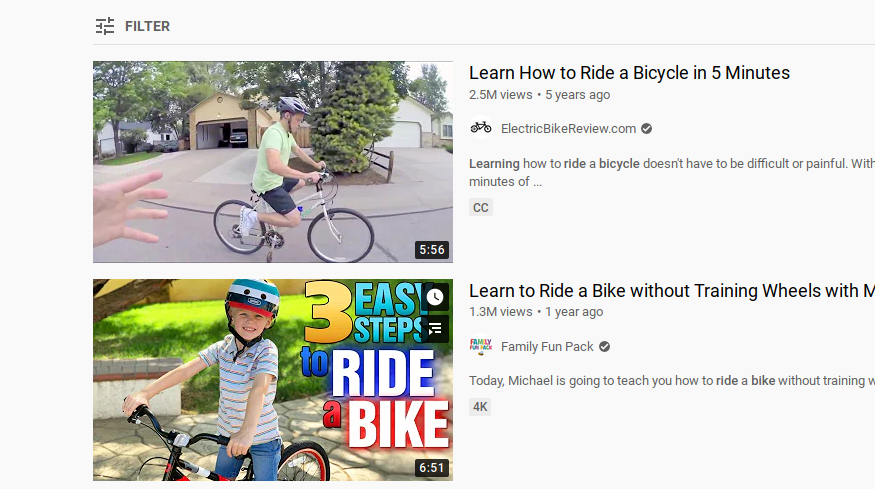
\includegraphics[scale=0.6]{learn.png} 

\end{frame}

\begin{frame}{Lectures}

   We will lectures that will cover the following aspects:

  \begin{itemize}
    \item Functional programming
\pause
    \item Operational semantics
\pause
    \item Higher order programming
\pause
    \item Complexity 
\pause
    \item Concurrency 
\pause
    \item Parallelism
  \end{itemize}

\vspace{20pt}\hspace{40pt} ... most lectures available as videos.  

\end{frame}

\begin{frame}{Assignments to pass the course}

  A set of hand in assignments.

  \vspace{20pt}\pause
  A short, 2-4 pages, report written in LaTeX following a template.

  \vspace{20pt}\pause
  No, not four pages of code!

  \vspace{20pt}\pause
  Explain what you did, why and what you learned.

\end{frame}


\begin{frame}{Assignments - deadline every Friday}

\begin{columns}
 \begin{column}{0.6\linewidth}
   To pass the course:
   \begin{itemize}
   \item Derivative - representing data, recursion. 
   \item A key-value store
   \item Evaluate an expression. 
   \item Towers of Hanoi
   \item Advent of Code 
   \item Monte Carlo
   \item Train shunting 
   \item Huffman coding
   \item ...???
   \end{itemize}
 \end{column}
 \begin{column}{0.4\linewidth}

   \pause
   For higher grades:
   \begin{itemize}
   \item Meta interpreter
   \item Higher order functions
   \item Advent of Code
   \item Dining philosophers
   \end{itemize}

 \end{column}
\end{columns}

\pause \vspace{20pt}
The seminars are not compulsory\pause\ \underline{handing in the report is.}

\end{frame}


\begin{frame}{course board}

  Two student representatives for course board. We will meet a couple
  of times during the course so that you can give feedback.

\end{frame}


\begin{frame}{finally}

  \pause\vspace{60pt}\hspace{40pt} Start programing today.

\end{frame}

\end{document}
